\documentclass[11pt]{article}
\usepackage[a4paper,bindingoffset=0.2in, left=1in,right=1in,top=1in,bottom=1in, footskip=.25in]{geometry}
%\documentclass[twocolumn,aps,pre]{revtex4}
%\usepackage[dvips]{graphicx}
\usepackage[french]{babel}
\usepackage[latin1]{inputenc}
\usepackage[OT1]{fontenc}
\usepackage{amsfonts}
\usepackage{epsfig}
\usepackage{graphicx}
%\usepackage{natbib}
\usepackage{amsmath}
\usepackage{amssymb}
\newcommand{\E}[1]{\mathbf{E}\left[#1\right] }

%debut

\begin{document}

\begin{center}
{\bf\Large HomeWork 2: Few simple problems}
\end{center}

This homework involves works on a computer, with the language of your choice. Present your result with graphs, plots, and data. Jupyter notebooks are a good option.


\section{Sampling $\pi$}

We come back to the problem of estimating $\pi$ by sampling uniformly points in the square between $-1<x<1$ and $-1<y<1$, and counting how many hits are inside the unit circle. For each points $i=1 \ldots N$, we define the random variable $S_i=0$ if the point is outside the circle, and $S_i=4$ if the point is inside the circle.

\begin{enumerate}
\item If each point $i$ is sampled uniformly in the square, what is the probability $p$ that $S_i=4$?
What are the mean $m$ and the variance $\Delta$ of the distribution $P(S_i)$?
\newline
\textbf{\underline{Answer :}}
\begin{eqnarray*}
S_i &= &4 \times U \quad \mbox{where} \quad U \quad \mbox{is a Bernoulli rv of parameter} \quad \frac{\pi}{4} \\
\E{S_i} &= &\pi\\
\mathrm{var}[S_i] &= &16\frac{\pi}{4}(1- \frac{\pi}{4}) \\
&= &\pi(4-\pi)
\end{eqnarray*}


\item If we are given $N$ perfectly random independent points, show that $\hat m$ and $\hat \Delta$ 
\begin{eqnarray}
\hat m = \frac 1N \sum S_i ~~~~
\hat \Delta = \frac 1{N-1} \sum S^2_i - {\hat m}^2 \nonumber
\end{eqnarray}
are unbiased estimates of the mean and variance of $P(S)$.
\newline
\textbf{\underline{Answer :}}
\begin{eqnarray*}
	\E{\hat m} &= &\frac{1}{N} N \E{S_i} \\
    N^2 \E{\hat m^2} &= &\sum_{ij} \E{S_i S_j} \\
    &= & \sum_{i} \E{S_i^2} + \sum_{i \neq j} \E{S_i S_j} \\
    &= &N \mbox{var}[S_i] + N\E{S_i}^2 + N(N-1)\E{S_i}^2 \\
    &= &N \mbox{var}[S_i] + N^2\E{S_i}^2 \\
    \E{\hat \Delta} &= &\frac{N}{N-1} \E{S_i^2 - \hat m^2} \\
    &= &\frac{N}{N-1} \left( \mbox{var}[S_i] + \E{S_i}^2 - \E{\hat m^2} \right) \\
    &= &\frac{N}{N-1} \left( \mbox{var}[S_i] + \E{S_i}^2 - \frac{1}{N}\mbox{var}[S_i] - \E{S_i}^2 \right) \\
    &= &\frac{N}{N-1} \frac{N-1}{N} \mbox{var}[S_i] \\
    &= &\mbox{var}[S_i]
\end{eqnarray*}


\item What is the variance of the estimator 
$\hat m$? Deduce the value of the typical error made by this estimator when using $N$ points to compute $\pi$.
\newline
\textbf{\underline{Answer :}}
\begin{eqnarray*}
	\mbox{var}[\hat m] &= &\E{\hat m^2} - \E{\hat m}^2 \\
    &= &\frac{\mbox{var}[S_i]}{N} \\
    &= &\frac{\pi(4 - \pi)}{N} \\
    \mbox{The typical error is} \quad \delta &= &\sqrt{\mbox{var}[\hat m_i]} = \sqrt{\frac{\pi(4 - \pi)}{N}}
\end{eqnarray*}


\item Implement the  sampling strategy where each points is selected uniformly in the square. Make a plot to make sure you are doing it well. For different values of $N$, compute $1000$ times different estimates of $\pi$. Check that the variance of your estimation is indeed close to the one predicted in Q.3. Compute the probability to make an error larger $0.01$ and compare with the various bounds we discussed in the course. 
\end{enumerate}
%

\section{Find the lighthouse}

A lighthouse is somewhere off a piece of straight coastline at a position $\alpha$ along the shore and a distance $\beta$ out at sea. It emits a series of short highly collimated flashes at random intervals and hence at random azimuths. These pulses are intercepted on the coast by photo-detectors that record only the fact that a flash has occurred, but not the angle from which it came. $N$ flashes have been recorded so far at positions $\{x_k\}$. Where is the lighthouse?

 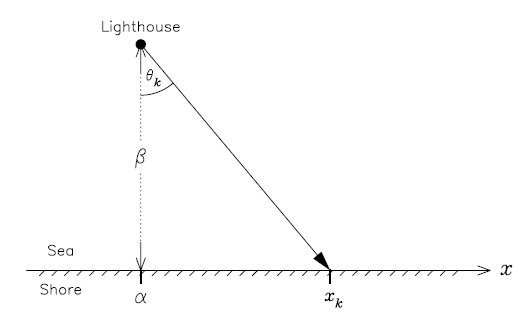
\includegraphics[width=0.5\textwidth]{download}

\begin{enumerate}
\item Show that the probability to observe an event at value $x_k$ is given by
$$
P(x_k ; \alpha,\beta) = \frac{\beta}{\pi \big[\beta^2 + (x_k - \alpha)^2 \big]}
$$
This  is known as a Cauchy or Lorentz distribution.
\newline
\textbf{\underline{Answer :}}
The procedure of sampling the angle $\theta_k$ is uniformly random between $-\frac{\pi}{2}$ and $\frac{\pi}{2}$ (we consider only the azimuths in front of the shore), we then have an uniform probability density $\frac{1}{\pi}$. Therefore we just perform a change of variable to $x_k$
\begin{eqnarray*}
	\frac{x_k - \alpha}{\beta} &= &\tan{\theta_k} \\
    \theta_k &= &\arctan{\frac{x_k - \alpha}{\beta}} \\
    \frac{d\theta_k}{dx_k} &= &\frac{1}{\beta(1 + \frac{x_k - \alpha}{\beta}^2)} \\
    &= &\frac{\beta}{ \big[\beta^2 + (x_k - \alpha)^2 \big]} \\
    P(x_k) &= &P(\theta_k) \times \frac{d\theta_k}{dx_k} \\
    &= &\frac{\beta}{\pi \big[\beta^2 + (x_k - \alpha)^2 \big]}
\end{eqnarray*}

\item Let us sample from it so that we can have some synthetic data to work with. Generate some synthetic data using the values $\alpha = 30.0$ and  $\beta = 10.0$. For instance $N=10$ points (most language do have a generator of random number from a Cauchy distribution).
\item Assume that the value of $\beta$ is known. Plot the likelihood (as a function of your estimated $\alpha$), together with a point indicating the 
the Maximum Likelihood estimate, for different values of $N$ between $10$ and $1000$.
\item Bonus question; when sampling the Cauchy distribution, does the mean coincides with the mode (i.e. the maximum) of the posterior? Why is that? Will they coincide in the $N \to \infty$ limit?
\newline
\textbf{\underline{Answer :}}
No it does not, and it will not coincide even in the $N \to \infty$ limit. This is because the mean value is not defined for the Cauchy distribution (first moment diverges).
\end{enumerate}
%

\section{Statistical inference and Maximum Likelihood}
%
We shall consider the problem discussed in our lecture, where a system emits particle with a half-length decay $\lambda$, which we detect if $1<\lambda<20$. The (density) probability to observe such a decay is thus
\begin{eqnarray}
P_{\lambda}(x_i) &=& \frac{e^{-x/\lambda}}{Z(\lambda)}~~\text{if $1<x<20$}\\
P_{\lambda}(x_i) &=& 0 ~~\text{otherwise} \nonumber
\end{eqnarray}

\begin{enumerate}
\item Compute $Z(\lambda)$ such that the probability is normalized. What the probability $P_{\lambda}(\left\{x\right\})$ to observe a set of $n$ events $(\left\{x\right\})$? Write a program that output $n$ such observation sampled from the probability distribution $(1)$.
\newline
\textbf{\underline{Answer :}}
\begin{eqnarray*}
	1 &= &\int_1^{20} \frac{e^{-x/\lambda}}{Z(\lambda)} dx\\
    &= &\frac{-\lambda}{Z(\lambda)} \left[ e^{-x/\lambda} \right]^{20}_1 \\
    &= &\frac{\lambda ( e^{-1/\lambda} - e^{-20/\lambda}) }{Z(\lambda)} \\
    Z(\lambda) &= &\lambda ( e^{-1/\lambda} - e^{-20/\lambda})
\end{eqnarray*}
\begin{equation*}
	P_\lambda (\left\{x\right\}) = \frac{e^{- \sum_{i=1}^n x_i/\lambda}}{Z(\lambda)^n} = \frac{e^{- \sum_{i=1}^n x_i/\lambda}}{\lambda^n ( e^{-1/\lambda} - e^{-20/\lambda})^n}
\end{equation*}



\item We choose the true value to be $\lambda^*=10$ . Generate $n=10$ observations. Plot the likelihood as a function of $\lambda$ and see how it is peaked arround the true value. Repeat for $n=100$ and $n=1000$.

\item We now assume that we are given a set of $n$ observations, without being told the true value of $\lambda$.  We consider the maximum likelihood estimator
\begin{eqnarray}
\hat \lambda_{\rm ML}(\left\{x\right\}) = \text{\rm argmax}_{\lambda} P_{\lambda}(\left\{x\right\})
\end{eqnarray}
and we shall define the squared error as  $\text{SE}=(\hat \lambda_{ML} (\left\{x\right\}) - \lambda)^2$. 

Create some data set with $n=10,100,1000$ for different values of $\lambda$ and see how the ML estimator performs. Note that finding the maximizer $\hat \lambda_{ML}$ can be done numerically 

\item If we average of many realizations of this process we can obtain the mean square error $MSE(\lambda,\hat \lambda,n)$, which is thus a function of $n$, $\lambda$ and of the estimator $\hat \lambda$. Compute, for instance for $n=10000$, the curve $MSE(\lambda,\hat \lambda_{\rm ML},n=10000)$. 

How does this curve compare with the Cramers-Rao bound ${\mathrm  {MSE}}({\hat  {\lambda }})\geq {\frac  {1}{I(\lambda )}}$, where $I(\lambda )$ is the total Fisher information. Is the ML estimator unbiased?
\newline
\textbf{\underline{Answer :}}

\end{enumerate}

%
\end{document}
%fin 
